% Created by tikzDevice version 0.12.3.1 on 2021-04-05 16:09:19
% !TEX encoding = UTF-8 Unicode
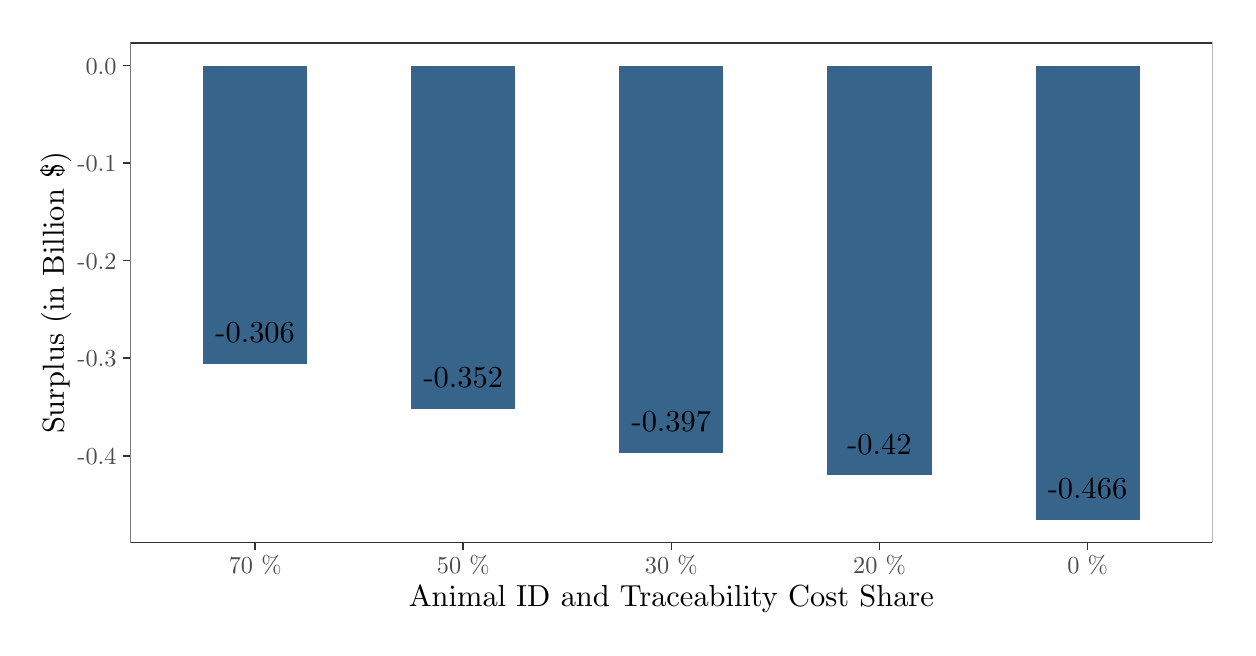
\begin{tikzpicture}[x=1pt,y=1pt]
\definecolor{fillColor}{RGB}{255,255,255}
\path[use as bounding box,fill=fillColor,fill opacity=0.00] (0,0) rectangle (433.62,216.81);
\begin{scope}
\path[clip] (  0.00,  0.00) rectangle (433.62,216.81);
\definecolor{drawColor}{RGB}{255,255,255}
\definecolor{fillColor}{RGB}{255,255,255}

\path[draw=drawColor,line width= 0.6pt,line join=round,line cap=round,fill=fillColor] (  0.00,  0.00) rectangle (433.62,216.81);
\end{scope}
\begin{scope}
\path[clip] ( 37.09, 30.69) rectangle (428.12,211.31);
\definecolor{fillColor}{RGB}{255,255,255}

\path[fill=fillColor] ( 37.09, 30.69) rectangle (428.12,211.31);
\definecolor{fillColor}{RGB}{54,100,139}

\path[fill=fillColor] (364.20, 38.90) rectangle (401.80,203.10);

\path[fill=fillColor] (289.00, 55.10) rectangle (326.60,203.10);

\path[fill=fillColor] (213.80, 63.21) rectangle (251.40,203.10);

\path[fill=fillColor] (138.61, 79.07) rectangle (176.21,203.10);

\path[fill=fillColor] ( 63.41, 95.27) rectangle (101.01,203.10);
\definecolor{drawColor}{RGB}{0,0,0}

\node[text=drawColor,anchor=base,inner sep=0pt, outer sep=0pt, scale=  1.10] at (383.00, 46.50) {-0.466};

\node[text=drawColor,anchor=base,inner sep=0pt, outer sep=0pt, scale=  1.10] at (307.80, 62.71) {-0.42};

\node[text=drawColor,anchor=base,inner sep=0pt, outer sep=0pt, scale=  1.10] at (232.60, 70.81) {-0.397};

\node[text=drawColor,anchor=base,inner sep=0pt, outer sep=0pt, scale=  1.10] at (157.41, 86.67) {-0.352};

\node[text=drawColor,anchor=base,inner sep=0pt, outer sep=0pt, scale=  1.10] at ( 82.21,102.88) {-0.306};
\definecolor{drawColor}{gray}{0.20}

\path[draw=drawColor,line width= 0.6pt,line join=round,line cap=round] ( 37.09, 30.69) rectangle (428.12,211.31);
\end{scope}
\begin{scope}
\path[clip] (  0.00,  0.00) rectangle (433.62,216.81);
\definecolor{drawColor}{gray}{0.30}

\node[text=drawColor,anchor=base east,inner sep=0pt, outer sep=0pt, scale=  0.88] at ( 32.14, 59.12) {-0.4};

\node[text=drawColor,anchor=base east,inner sep=0pt, outer sep=0pt, scale=  0.88] at ( 32.14, 94.36) {-0.3};

\node[text=drawColor,anchor=base east,inner sep=0pt, outer sep=0pt, scale=  0.88] at ( 32.14,129.60) {-0.2};

\node[text=drawColor,anchor=base east,inner sep=0pt, outer sep=0pt, scale=  0.88] at ( 32.14,164.83) {-0.1};

\node[text=drawColor,anchor=base east,inner sep=0pt, outer sep=0pt, scale=  0.88] at ( 32.14,200.07) {0.0};
\end{scope}
\begin{scope}
\path[clip] (  0.00,  0.00) rectangle (433.62,216.81);
\definecolor{drawColor}{gray}{0.20}

\path[draw=drawColor,line width= 0.6pt,line join=round] ( 34.34, 62.15) --
	( 37.09, 62.15);

\path[draw=drawColor,line width= 0.6pt,line join=round] ( 34.34, 97.39) --
	( 37.09, 97.39);

\path[draw=drawColor,line width= 0.6pt,line join=round] ( 34.34,132.63) --
	( 37.09,132.63);

\path[draw=drawColor,line width= 0.6pt,line join=round] ( 34.34,167.86) --
	( 37.09,167.86);

\path[draw=drawColor,line width= 0.6pt,line join=round] ( 34.34,203.10) --
	( 37.09,203.10);
\end{scope}
\begin{scope}
\path[clip] (  0.00,  0.00) rectangle (433.62,216.81);
\definecolor{drawColor}{gray}{0.20}

\path[draw=drawColor,line width= 0.6pt,line join=round] ( 82.21, 27.94) --
	( 82.21, 30.69);

\path[draw=drawColor,line width= 0.6pt,line join=round] (157.41, 27.94) --
	(157.41, 30.69);

\path[draw=drawColor,line width= 0.6pt,line join=round] (232.60, 27.94) --
	(232.60, 30.69);

\path[draw=drawColor,line width= 0.6pt,line join=round] (307.80, 27.94) --
	(307.80, 30.69);

\path[draw=drawColor,line width= 0.6pt,line join=round] (383.00, 27.94) --
	(383.00, 30.69);
\end{scope}
\begin{scope}
\path[clip] (  0.00,  0.00) rectangle (433.62,216.81);
\definecolor{drawColor}{gray}{0.30}

\node[text=drawColor,anchor=base,inner sep=0pt, outer sep=0pt, scale=  0.88] at ( 82.21, 19.68) {70 \%};

\node[text=drawColor,anchor=base,inner sep=0pt, outer sep=0pt, scale=  0.88] at (157.41, 19.68) {50 \%};

\node[text=drawColor,anchor=base,inner sep=0pt, outer sep=0pt, scale=  0.88] at (232.60, 19.68) {30 \%};

\node[text=drawColor,anchor=base,inner sep=0pt, outer sep=0pt, scale=  0.88] at (307.80, 19.68) {20 \%};

\node[text=drawColor,anchor=base,inner sep=0pt, outer sep=0pt, scale=  0.88] at (383.00, 19.68) {0 \%};
\end{scope}
\begin{scope}
\path[clip] (  0.00,  0.00) rectangle (433.62,216.81);
\definecolor{drawColor}{RGB}{0,0,0}

\node[text=drawColor,anchor=base,inner sep=0pt, outer sep=0pt, scale=  1.10] at (232.60,  7.64) {Animal ID and Traceability Cost Share};
\end{scope}
\begin{scope}
\path[clip] (  0.00,  0.00) rectangle (433.62,216.81);
\definecolor{drawColor}{RGB}{0,0,0}

\node[text=drawColor,rotate= 90.00,anchor=base,inner sep=0pt, outer sep=0pt, scale=  1.10] at ( 13.08,121.00) {Surplus (in Billion \$)};
\end{scope}
\end{tikzpicture}
